\chapter{Statistiques}
   \minitoc
      \section{Généralités}

      Dans le cadre de notre projet, nous allons effectuer quelques analyses statistiques avec l'ensemble des données fournies.
      
      Dans cette perspective nous allons clarifier quelques termes nécessaires à la bonne compréhension de notre analyse.
      \section{Analyse descriptive}
        L'analyse descriptive est un sous-domaine des méthodes quantitatives (méthodes de recherches scientifiques utilisant l'analyse mathématique et scientifique). Dans la perspective d'appliquer cette science à notre base de données, nous allons par la suite nous inspirer de la statistique descriptive, afin de caractériser différentes catégories d'élèves 

         
         \subsection{Algorithmes et explication pédagogiques}
         
         Afin de choisir les outils statistiques pertinentes aux données fournies, on s'est inspiré des données fournies par le site \textbf{www.scei-concours.fr}.
         Nous allons donc nous intéresser à l'implémentation de fonctions Python permettant le calcul de ces données ainsi que des fonctions complémentaires dont nous allons montrer l'algorithme ci-dessous.
          \begin{center}
         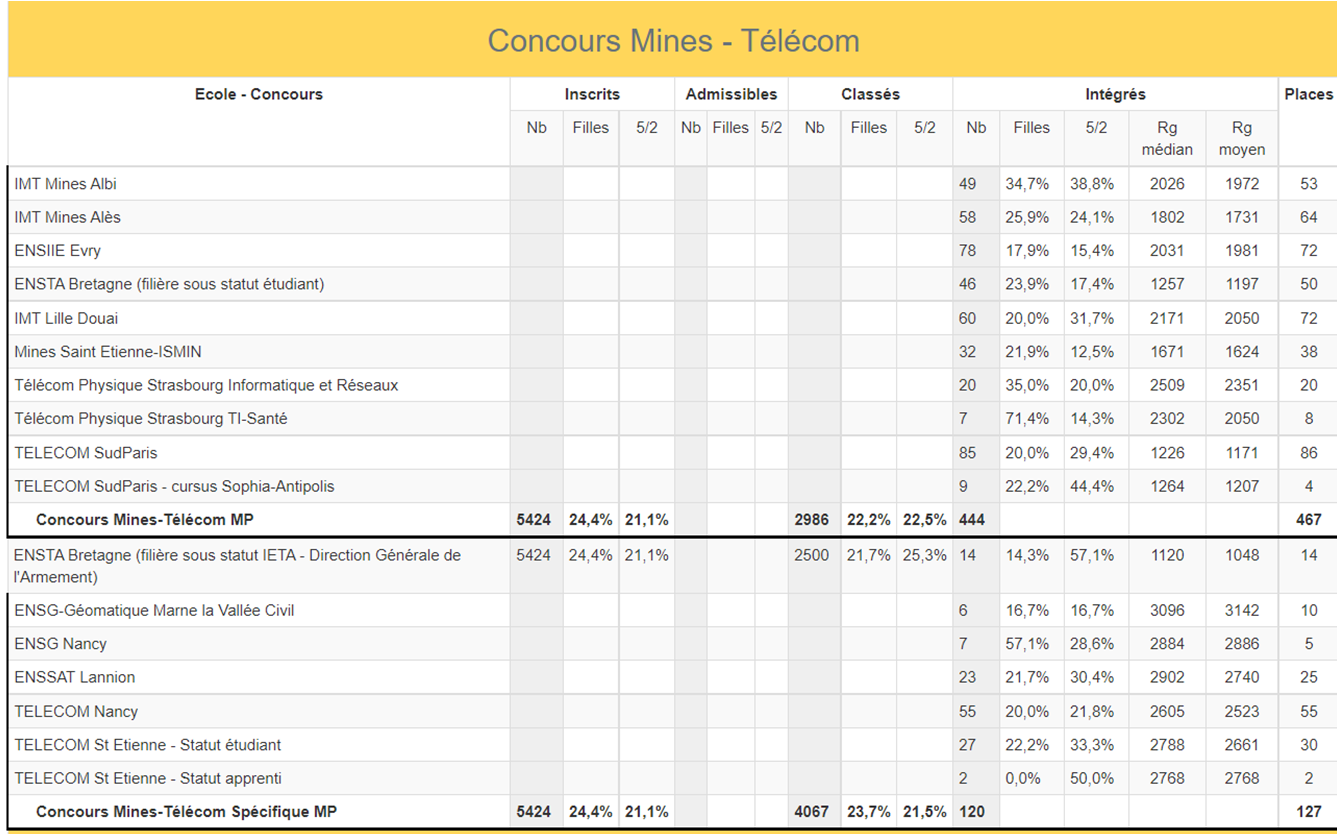
\includegraphics[width=15cm]{statimt.png}\\
         \textbf{Figure1:} Tableaux des statistiques 2020 sur scei (ici filière MP)
         \end{center}
         
         \subsubsection{Dispersion : Variance}
         La dispersion représente la variabilité des différentes valeurs que peut prendre une variable. En statistiques, il existe différentes mesures de la dispersion. Les plus courantes sont la variance, l'écart-type ou encore l'intervalle inter-quartile. C'est une mesure peu influencée par la présence de valeurs extrêmes.\\
        
        La variance est la moyenne des carrés des écarts à la moyenne:\\
        \[\sigma^2 = \frac{\displaystyle\sum_{i=1}^{n}(x_i - \mu)^2} {n} \]
        Il s'agit alors d'appliquer l'algorithme ci-dessous:\\
        
         \begin{algorithm}[H]
         \SetAlgoLined
         \KwResult{Variance}
          l=list()\;
          \For{i=0 jusqu'à la longueur de la liste l avec un pas de 1}{
           compteur=0\;
          \For{j=0 jusqu'à la longueur de la liste l avec un pas de 1}{
           \If{l(i)(j)=n}{
           compteur=compteur+1;}\
     
         }
         l=l+compteur;}
         compteur=0;\\
         \For{i=0 jusqu'à la longueur de la liste l avec un pas de 1}{
         compteur=compteur+l(i);}
         moyenne=compteur/longueur(l);\\
         compteur=0;\\
         \For{i=0 jusqu'à la longueur de la liste l avec un pas de 1}{
         compteur=compteur+($l(i)-moyenne)^2$\\ }
         Variance=compteur/longueur(l);
         
         
 \caption{Variance}
\end{algorithm}
\subsubsection{Dispersion : Ecart-type}
 L'Ecart-type est la moyenne quadratique des écarts par rapport à la moyenne ou plus simplement la racine carrée de la Variance:\\ \[\sigma = \sqrt\frac{\displaystyle\sum_{i=1}^{n}(x_i - \mu)^2} {n} \]\\
 En admettant la viabilité de l'algorithme précédent, on définie une unique instruction: l'attribution de la racine carrée de la valeur absolu du résultat obtenu par l'algorithme précédent.\\
 
        \begin{algorithm}[H]
         \SetAlgoLined
         \KwResult{Et }
          Et=$\sqrt{|Variance|}$;\;
          
 \caption{Ecart-type}
\end{algorithm}

\subsubsection{Médiane}

La médiane d'un ensemble de valeurs (échantillon, population,
distribution de probabilités) est une valeur m qui permet de couper
l'ensemble des valeurs triées en deux parties égales : mettant d'un côté
une moitié des valeurs, qui sont toutes inférieures ou égales à m et de
l'autre côté l'autre moitié des valeurs, qui sont toutes supérieures ou
égales à m (s'il y a un nombre pair de valeurs, la médiane sera la
moyenne des 2 valeurs "centrales" de la distribution): \\

    Si l'effectif total de la série est impair: $N=2p+1$, 
  la médiane est la $(p+1)^{\text{ème}}$ valeur.\;

  Si l'effectif est pair: $N=2p$, on prend en général pour médiane la
  moyenne de la $p^{\text{ème}}$ et de la $(p+1)^{\text{ème}}$ valeur. \\
  
  Il s'agit alors d'appliquer l'algorithme ci-dessous:\\

         \begin{algorithm}[H]
         \KwResult{Mediane }
          Med=list();\\
          \For{i=0 jusqu'à la longuer de la liste l avec un pas de 1}{
           med=med+liste(i)\;}
         \textbf{end}\\  
         N=entier((longueur(med)+1/2);\\
         med=sorted(med);\\
         mediane=0
         \eIf{longueur(Mediane){$\equiv 0 \mod 2$}}{mediane=med(longueur(med)+1/2)+longueur((med)-1/2)/2;}{ mediane=med(N);}
         
         \textbf{end}
         
         \caption{Mediane}
         
        \end{algorithm}
        \subsubsection{Premier Quartile}
        Les quartiles sont les 3 valeurs qui divisent les données triées en 4 parts égales, de sorte que chaque partie représente 1/4 de l'échantillon de la population. Il existe donc trois quartiles : Q1, Q2 (égal à la  médiane) et Q3. Par exemple, Q1 est la valeur telle que 25 \% des valeurs de l'échantillon lui sont inférieures, 75 \% supérieures.\\
        
         \begin{algorithm}[H]
         \KwResult{Premier Quartile }
          premquart=list();\\
          \For{i=0 jusqu'à la longueur de la liste avec un pas de 1}{
           premquart=prequart+liste(i)\;}
         \textbf{end}\\  
         N=entier((longueur(premquart))//4)\\
         premquart=sorted(premquart);\\
         Premier Quartile=0\\
         \eIf{longueur(premquart){$\equiv 0 \mod 4$}}{Premier Quartile=premquart(longueur(premquart)//4-1);}{ Premier Quartile=premquart(N);}
         
         \textbf{end}
         
         \caption{Premier Quartile}
         
        \end{algorithm}
\section{Modélisation et représentation des résultats statistiques}
Ils existent plusieurs façons de modéliser et d'exprimer les résultats des statistiques qui nous intéressent. Que ça soit des données pures organisées sous forme de tableau ou encore des cartes interactives . Nous avons décidé de garder le format scei qui semble être optimale, pour le service rendu.